\documentclass{beamer}
%% Possible paper sizes: a0, a0b, a1, a2, a3, a4.
%% Possible orientations: portrait, landscape
%% Font sizes can be changed using the scale option.
\usepackage[size=a3,orientation=portrait,scale=1.8]{beamerposter}
\usetheme{LLT-poster}
\usecolortheme{ComingClean}
% \usecolortheme{Entrepreneur}
% \usecolortheme{ConspiciousCreep}  %% VERY garish.

\usepackage[utf8]{inputenc}
\usepackage[T1]{fontenc}
\usepackage{libertine}
\usepackage[scaled=0.92]{inconsolata}
\usepackage[libertine]{newtxmath}
\usepackage[numbers]{natbib}
\renewcommand{\bibfont}{\small}

\newcommand{\texthash}{\#}


%% Load the markdown package
\usepackage[citations,footnotes,definitionLists,hashEnumerators,smartEllipses,tightLists=false,pipeTables,tableCaptions,hybrid]{markdown}
%%begin novalidate
\markdownSetup{rendererPrototypes={
 link = {\href{#2}{#1}},
 headingFour = {\begin{block}{#1}},
 horizontalRule = {\end{block}}
}}
%%end novalidate

\author[Chevalier.V]{mecacorbu.odoo.com/}
\title{STS CPRP $2^{eme}$ année}
\institute{Lycée Le Corbusier}
% Optional foot image
\footimage{
\includegraphics[width=4cm]{logo1.png}}

\begin{document}

\begin{frame}[fragile]\centering

\textbf{\textit{Résumé paramètre de coupe}}

\begin{columns}
\begin{column}{0.57\textwidth}

\begin{markdown}

#### Rugosité $R$ ($\mu m$)

- Rugosité $\equiv$ état de surface
- Sans indication, norme ISO 2768mk : 3,2 $\mu m$
- $R_a$ rugosité arithmétique
- $R_t$ rugosité de profondeur
- Rugosité + faible si : $f_z$ $\searrow$, $\varnothing$ rayon de bec $\nearrow$, mocn rigide.
- Rugosité + grande si : vibration $\nearrow$, $N$ $\nearrow$, $f_z \nearrow$, mocn flexible.
- Une bonne rugosité dépend d'un plan d'expérience et il y aura toujours des compromis entre les paramètres et les matières des outils et du brut.


----
\end{markdown}
\begin{figure}
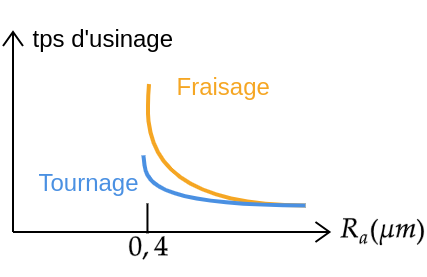
\includegraphics[width=0.4\textwidth]{courbe1.png}
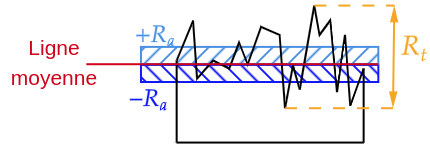
\includegraphics[width=0.4\textwidth]{Ra1.png}
\end{figure}
\end{column}




\begin{column}{.4\textwidth}
\begin{markdown}




#### Avance $f$ (mm/tour) [Tournage]

- $f$ $\Rightarrow$ temps d'usinage
- $f=\frac{V_f}{N}$
- Exemple : pour un brut en aliage d'aluminium et un outil en carbure $f \simeq 0,2 \sim 0,4$ mm/tour

----
\end{markdown}
\begin{figure}
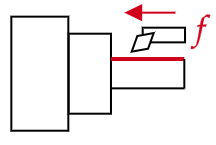
\includegraphics[width=0.3\textwidth]{f1.png}
\end{figure}

\end{column}

\end{columns}

\bigskip

\begin{columns}[T]

%%%% First Column
\begin{column}{.46\textwidth}

\begin{markdown}

#### $f_z$ Avance par dent (mm/tour/dent)

- Pour le fraisage
- $f_z = \frac{Vf}{Z.N}$
- Exemple : pour un brut en S235 et un outil en ARS : $0,05 \leq f_z \leq 0,11$ mm/tour/dent.
- pour un brut en S235 et un outil en carbure : $0,07 \leq f_z \leq 0,2$ mm/tour/dent.

----

\begin{figure}
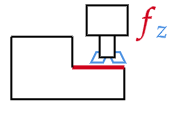
\includegraphics[width=0.3\textwidth]{fz1.png}
\end{figure}

#### Vitesse d'avance $V_f$ (mm/min)

- $V_f=Z.fz.N$
- La vitesse d'avance se calcul en fonction des autres paramètres

\setkeys{Gin}{width=.3\linewidth}



----


\end{markdown}



\end{column}









%%%% Second Column
\begin{column}{.46\textwidth}

\begin{markdown}

#### Vitesse de coupe $V_c$ (mètre/min)

- Un identifiant et un mot de passe vous seront donnés. Lors de votre première connexion, vous devrez \textbf{redéfinir un nouveau mot de passe}. Pensez à bien noté, ou \textbf{prendre en photo} l'identifiant et le \textit{nouveau mot de passe}, car il sera difficile de les récupérer rapidement.

----

#### Fréquence de rotation $N$ (tour/min)

- D’une manière générale, vos fichiers doivent être compréhensible et identifiable. Nous devons savoir quel est le nom du devoir, et le ou les prénoms/noms. Si vous faite un devoir de dessin industriel, vous pouvez enregistrer vos devoirs de cette façon :

- \textbf{Dessin-definition-1-Nom-Prenom.catDrawing}

----


\end{markdown}
\end{column}
\end{columns}


\bigskip
{\usebeamercolor[bg]{headline}\hrulefill}
\bigskip

\begin{markdown}

#### Informations complémentaires

- $Z$ : nombre de dent
- ARS : Outil "Acier Rapide Supérieur"
- S235 : Acier doux étiré à froid

----

\end{markdown}

\end{frame}


\end{document}